\documentclass{article}
\usepackage[T1]{fontenc}
\usepackage{lmodern}
\usepackage{graphicx}
\usepackage{amsmath,amssymb}
\usepackage[a4paper,margin=2cm]{geometry}
\usepackage[absolute,overlay]{textpos}
\setlength{\TPHorizModule}{1mm}
\setlength{\TPVertModule}{1mm}
\usepackage[indonesian]{babel}
\usepackage{hyperref}
\setlength{\emergencystretch}{2em}
% unit: Halaman 6

\begin{document}

% === Halaman 6 (python/native) ===

Rinaldi M/II4020 Kriptografi

6

Hybrid Cryptography

https://www.researchgate.net/figure/Illustration-of-a-hybrid-

cryptosystem\_fig8\_327799148

% deskripsi: gambar native xref 39
\noindent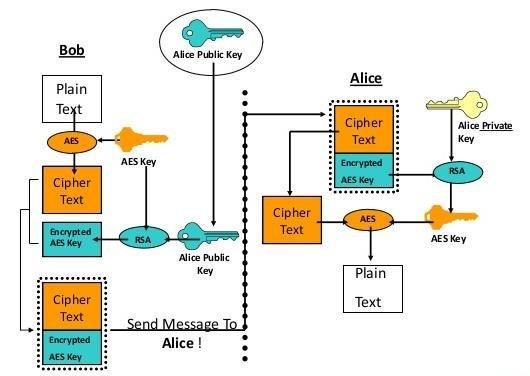
\includegraphics[width=0.85\textwidth]{../../images/python/page_006_img_01.jpeg}

\end{document}
